\chapter{Exécution}

\begin{center}
    \makebox[\textwidth]{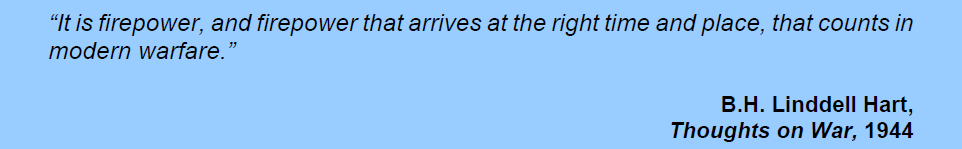
\includegraphics[width=\paperwidth]{quote5.png}}
\end{center}

\section{Introduction}

L'exécution du \gls{cas} commence lorsque la cible est désignée par le \gls{gc} soutenu, et décrit les considérations à prendre en compte pour intégrer le \gls{cas} aux manoeuvres de l'unité soutenue.

\section{Engagement de la cible lors du CAS}

Cette section décrit les procédures standard lors du \gls{cas}. Bien que certaines opérations nécessitent des procédures spécifiques, le personnel impliqué dans le \gls{cas} doit être familier avec le format standard.

\subsection{Création du briefing par le J-TAC}
Cette sous-section décrit les tâches que doit effectuer le \gls{jtac} une fois que la cible a été désignée par le \gls{gc}.

\e
    \item Rassembler les informations à propos de la cible
    \ee
        \itemt{Élévation de la cible (ligne 4)}{
        Par défaut, l'élévation est exprimée en pieds au dessus de la mer (ft \gls{msl})}
        \itemt{Description de la cible (ligne 5)}{
        La description de la cible doit être concise et précise (par ex. ``5 chars dans un champ''). Le \gls{jtac}/\gls{faca} doit éviter d'utiliser des descriptions compliquées ou des termes qui risquent de ne pas être compris par les pilotes. Cependant, la descrition doit rester spécifique. si le \gls{gc} veut attaquer une \gls{hvt} qui se trouve dans un building à deux étages, il devra spécifier "\gls{hvt} dans building à 2 étages", et pas seulement "building à 2 étages".}
        \itemt{Position de la cible (ligne 6)}{
        Le \gls{jtac}/\gls{faca} doit évaluer la précision minimale nécéssaire pour les coordonnées de la cible pour accomplir les objectifs du \gls{gc}. Un largage de bombe guidée laser depuis un émetteur au sol demandera des coordonnées beaucoup moins précises qu'une largage de \gls{jdam}.}
        \eee
            \itemt{Association du terrain et d'une carte}{
            Le moins précis, mais rapide et efficace en fonction de la situation.}
            \itemt{\gls{lrf} couplé au \gls{gps} et/ou la boussole}{
            Sujet à l'imprécision de la boussole, et au brouillage \gls{gps}. Si le brouillage \gls{gps} est possible, une autre méthode devra être utilisée.}
            \item Logiciel de ciblage
            \item Coordonnées dérivées des images de reconnaissance
        \ed
        \itemt{Positions alliées (ligne 8)}{
        La positions des unités alliées au sol sont données à partir de la position de la cible. La direction est donnée de manière cardinale ou sous-cardinale, et la distance est exprimée en mètres. L'observateur ou le \gls{jtac} peuvent ne pas être l'unité alliée la plus proche de la cible.}
        \itemt{Effet souhaité par le \gls{gc}}{
        L'effet souhaité par le \gls{gc} est déterminé en parlant avec lui. Le \gls{jtac} doit offrir au \gls{gc} une estimation réaliste des possibilités en fonction des appareils disponibles, de l'armement embarqué, et de son expertise.}
    \ed
\ed
\subsection{Requête de CAS}
\e
    \item Une fois que la position de la cible a été grossièrement estimée, le \gls{jtac} doit envoyer la demande de \gls{cas} le plus vite possible, pour prendre en compte le temps nécessaire avant l'arrivée des appareils. Il ne faut pas retarder l'envoi de la demande pour augmenter la précision des coordonnées de la cible.\\ \important{Il ne faut jamais utiliser les coordonnées des unités alliées comme coordonnées cible dans une demande de \gls{cas}.}
    \itemt{Création du game plan}{
    Au minimum, le game plan contiendra le type de contrôle et la méthode d'attaque. D'autres informations peuvent être intégrée au game plan ou être ajouté plus tard aux remarques du CAS brief: les intentions du \gls{gc}, l'effet désiré, l'intervalle entre les appareils dans le cas d'une attaque simultanée par plusieurs éléments \gls{cas}. Dans le cas d'attaques séquentielles (\gls{sead}, marquage), une attention particulière devra être apportée à l'établissement de la séparation entre les appareils. L'objectif du \gls{jtac} n'est pas de dicter aux appareils de \gls{cas} les tactiques à employer, mais de fournir un plan qui correspond aux intentions du \gls{gc}.}
    \ee
        \itemt{Déterminer l'effet désiré}{
        \remark{
        \eee
            \item Composition de la cible (blindage)
            \item Répartition de la cible (centré sur un point ou dispersé)
            \item Position (dégagée ou protégée)
            \item Dégâts collatéraux potentiels
            \item Proximité des unités alliées
        \ed}}
        \itemt{Choisir le type de \gls{tac}}{
        Le type de \gls{tac} dépend de l'armement employé, de la manière manière de réduire les risques, de la vitesse de l'engagement et de la capacité du \gls{jtac} à voir la cible et/ou l'appareil qui attaque.}
        \itemt{Choisir la méthode d'attaque (\gls{boc} ou \gls{bot})}{
            La méthode d'attaque est choisie de manière à permettre l'attaque la plus rapide possible, en fonction du type de cible, de la façon dont sera acquise la cible, et de la situation}
        \itemt{Planifier l'intervalle entre les appareils}{
        Le \gls{jtac} peut demander un intervalle spécifique entre les attaques, en fonction de la cible, des menaces, des activités alliées, de la déconfliction artillerie/\gls{sead}/laser, de l'armement utilisé, des restrictions, de la météo, etc. Les pilotes se doivent d'adapter leur tactiques pour respecter le timing et les intervalles imposés.}
        \eee
        	\itemt{Attaque simultanée}{
        	Tous les appareils délivreront leur armement de manière à créer un effet simultané. Cette méthode minimise l'exposition des appareils aux menaces et offre à l'ennemi un temps de réaction très court. C'est la méthode optimale pour engager des cibles multiples, tout particulièrement des cibles mobiles qui pourraient fuir après la première attaque. Le principal désavantage de cette méthode est l'impossibilité de corriger ou d'annuler le tir entre les impacts et la diminution du support mutuel entre les appareils qui attaquent.\\
        	\important{Un attaque simultanée nécessite que les appareils utilisent des codes laser différents.}}
        	\itemt{Attaque séquentielle}{
        	Les appareils attaquent un à la fois, avec un intervalle spécifique entre les attaques, basé sur le temps nécessaire à l'acquisition de l'appareil précédent, la durée de vol de l'arme employée, le temps nécessaire au dégagement visuel de la zone attaquée (fumée, fragments, etc.), et le temps nécessaire à évaluer l'efficacité de la frappe précédente et le besoin d'une nouvelle frappe.\\ Quelques guides pour les attaques séquentielles:
        	\eeee
        		\item 30 secondes pour un contrôle de \gls{typeone} avec des bombes lisses
        		\item 1 minute pour des \gls{lgb} délivrées à altitude moyenne
        		\item Plus de deux minutes pour décider de la ré-attaque lors de l'emploi de \gls{pgm} à haute ou moyenne altitude
        	\ed}
        \ed
    \ed
    \item Détermination du type de marque et de l'aide à la corrélation
    \ee
    	\itemt{\gls{boc}}{
    	\eee
    		\item Pas de marque nécessaire (ligne 7: "No mark")
    		\item Si le \gls{tac} est utilisé avec des \gls{lgw}, le call-sign de l'unité qui fournit le \gls{tac} et le code laser seront fournis.\\ (ligne 7 (exemple): "Blackjack laser, code 1688")
    	\ed}
    	\itemt{\gls{bot}}{
    	La marque dépendra de l'appareil qui attaque}
    	\item \gls{bot} et contribution d'une tierce partie
    	\eee
    		\itemt{Tierce partie}{
Suite l'expansion des technologies déployées sur le champ de bataille, le \gls{jtac} peut décider de recourir à une tierce partie (unité \gls{recce}, sniper, appareils équipés d'un émetteur laser, etc.) pour aider à l'obtention des coordonnées ou de la position de la cible, à l'attaque terminale ou à l'établissement du \gls{bda}. De ce fait, la corrélation avec ces parties tierces sera également nécessaire.}
\item Considérations
			\eeee
				\item Les pilotes utilisent généralement une combinaison de senseurs et leurs yeux pour acquérir les marques et les cibles. Le \gls{jtac} doivent être familiers avec les capacités des senseurs et utiliser des marques qui utilisent ces capacités.
				\item Le \gls{jtac} doit toujours avoir en réserve un plan de marquage alternatif.
			\ed
			\item Types de marque et \gls{tgo}
			\eeee
				\itemt{Marquage laser}{
				Le passage de la marque laser est le fait d'utiliser un \gls{ltd} pour fournir l'énergie laser au \gls{lst} de l'appareil. Le \gls{ltd} peut se trouver au sol ou embarqué dans un autre appareil.}
				\eeeee
					\item Avantages
					\eeeeee
						\item Excellente corrélation de la position de la cible si la géométrie correcte est utilisée
						\item Peut être utilisé de jour comme de nuit
					\ed
					\item Désavantages
					\eeeeee
							\item Nécessite un \gls{ltd} et un \gls{lst}
							\item Demande de la coordination géométrique pour le \gls{lst} ne traque pas le \gls{ltd} (l'origine du pointage)
							\item Le marquage laser depuis le sol est souvent difficile, particulièrement lorsque l'unité qui effectue le pointage est sous le feu ennemi
							\item Un premier passage d'acquisition de la marque est parfois nécessaire
					\ed
				\important{Lors du marquage laser depuis le sol, un \gls{fah} sera obligatoirement donné, de manière à renforcer l'établissement de la géométrie correcte}
				\ed
				\itemt{Marquage infrarouge (\acrshort{sparkle})}{
				Les pilotes utiliseront leur \gls{nvg} pour acquérir la cible.\\
				\important{Les pilotes doivent appeler "VISUEL SPARKLE", "TALLY SPARKLE" ou "CONTACT SPARKLE" quand un marquage infrarouge est utilisé à partir du sol}
				\eeeee
					\item Avantages
					\eeeeee
						\item Rapide
						\item Le \gls{jtac} a la confirmation visuelle que le pilote a bien acquis la cible correcte							
					\ed
					\item Désavantages
					\eeeeee
						\item De nuit seulement
						\item Requiert de la coordination géométrique pour s'assurer que le pilote a bien acquis la fin du faisceau infrarouge et non pas sa source
						\item S'il y a plusieurs pointeurs \gls{ir} près d'une même cible, il devient difficile pour le \gls{jtac} de déterminer si le pointeur se trouve bien sur la cible à cause du phénomène de ``diffusion'' dans les \gls{nvg}
						\item Si l'ennemi dispose également de \gls{nvg}, l'utilisation d'\gls{ir} expose l'opérateur et supprime le facteur de surprise
					\ed
				\ed}
				\itemt{Marquage à partir d'un \gls{trp}}{
				\eeeee
					\item Avantages
					\eeeeee
						\item Prêt rapidement si le pilote connaît le \gls{trp}
						\item De jour comme de nuit
						\item Offre un point de référence commun pour le talk-on
					\ed
					\item Désavantages
					\eeeeee
						\item Nécessite le pilote connaisse le \gls{trp}
					\ed
				\ed}
				\itemt{Marquage \gls{idf} (fumigène)}{
				\eeeee
					\item Avantages
					\eeeeee
						\item De jour comme de nuit (obus phosphorescents ou lumineux)
						\item Le \gls{jtac} ne doit pas dévoiler sa position
						\item Offre un point de référence commun pour le talk-on
					\ed
					\item Désavantages
					\eeeeee
						\item Prend du temps à coordonner
						\item Le manque de précision implique souvent une correction supplémentaire à partir de la marque
						\item Le tire indirect implique une déconfliction supplémentaire
						\item Le \gls{fov} des senseurs peut être un problème si la marque se trouve en dehors
						\item L'illumination de nuit sature les \gls{nvg}
						\item Sacrifie l'effet de surprise
					\ed
				\ed}
				\itemt{Marquage par feu direct}{
				Utilise un tir direct (munitions traçantes ou grandes fumigènes) pour marquer la cible
				\eeeee
					\item Avantages
					\eeeeee
						\item Facilement accessible
					\ed
					\item Désavantages
					\eeeeee
						\item Risque de dommages collatéraux
						\item Difficulté pour les \gls{rw} d'acquérir visuellement la marque de jour
						\item Difficulté pour les \gls{fw} d'acquérir visuellement la marque de jour comme de nuit
						\item Le \gls{fov} des senseurs peut être un problème si la marque se trouve en dehors
						\item L'illumination de nuit sature les \glspl{nvg}
						\item Sacrifie l'effet de surprise
					\ed
				\ed}
				\itemt{Considérations pour le marquage de nuit}{
				\eeeee
					\item La visibilité limitée et le manque de perspective rend la corrélation de nuit difficile
					\item L'illumination du champ de bataille doit être planifiée de manière à ne pas saturer les \glspl{nvg}
				\ed}
				\itemt{Marques d'opportunité}{
				N'importe quoi sur le champ de bataille peut servir de marque; un bâtiment en feu, le trafic routier, etc.}
			\ed
       	\ed
    \ed
    \item Détermination la géométrie d'attaque reprise 227 TODO
\ed


\e
    \item Déroulement d'une mission \gls{cas}:
    \begin{figure}[H]
        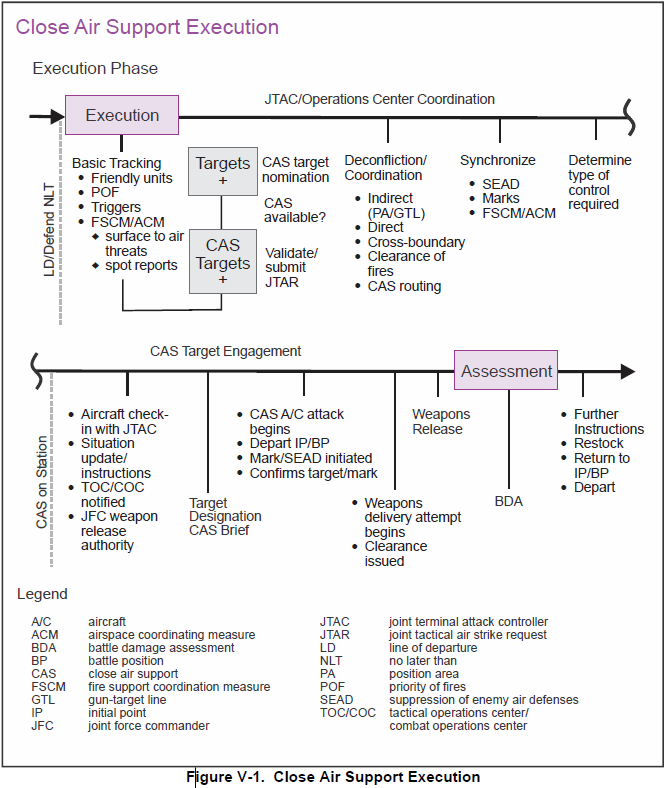
\includegraphics[width=\textwidth]{execution-full.png}
        \caption{Déroulement d'une mission.}
        \label{fig:casflow-full}
    \end{figure}
    \item Cas flow simplifié:
    \begin{figure}[H]
        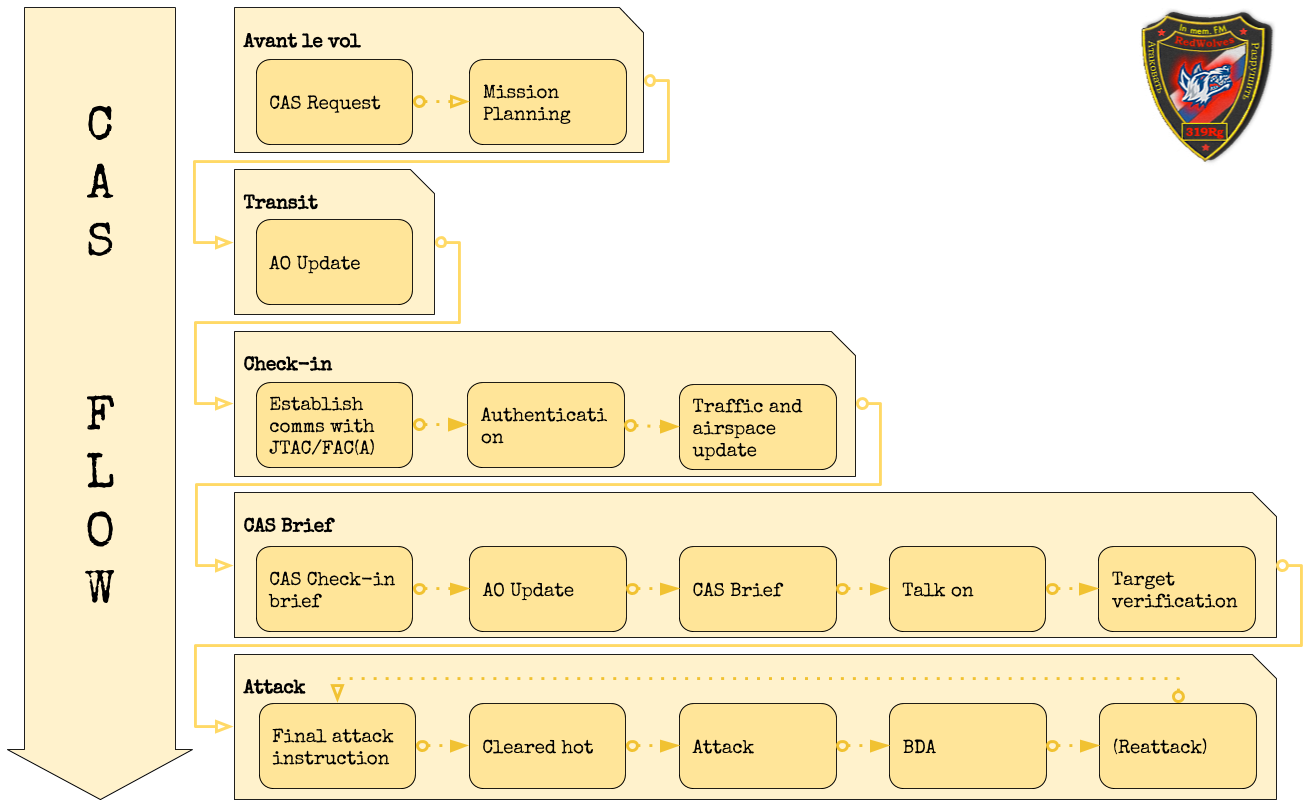
\includegraphics[width=\textwidth]{CASFlow.png}
        \caption{Cas flow simplifié.}
        \label{fig:casflow}
    \end{figure}
\ed

\e
    \item
    Ce chapitre présente le déroulement pratique d’une mission \acrshort{cas}. Le template qui y est présenté illustre une mission \acrshort{cas} typique, et fournit un guide pour le \acrshort{jtac}/\acrshort{faca} et le pilote pour les aider à remplir leur mission.
    \item Le déroulement présenté ici commence après le décollage, et se termine lorsque la patrouille de \acrshort{cas} est sur le retour.
\ed

\section{Routing}
\e
    \item Le routing consiste à diriger les appareils d’un point à un autre.
    \item Extrait du \jp:\\
    \begin{figure}[H]
        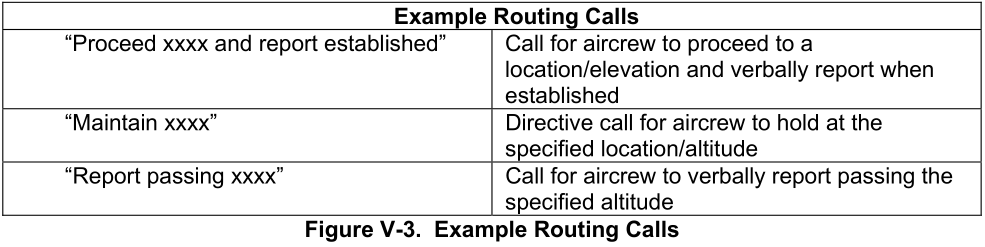
\includegraphics[width=\textwidth]{routing.png}
        \caption{Routing.}
        \label{fig:routing}
    \end{figure}
    \item Exemples:\\
    \ee
        \item Routing standard, demande de maintien de position:\\
        \begin{figure}[H]
            
\includegraphics[width=\textwidth]{routing_ex1.png}
            \caption{Routing: maintien de position.}
            \label{fig:routingpos}
        \end{figure}
        \item Si le contrôleur n'est pas certain de la position et de l'altitude de l'appareil, il doit demander les informations:\\
        \begin{figure}[H]
            
\includegraphics[width=\textwidth]{routing_ex2.png}
            \caption{Routing: demande d'information.}
            \label{fig:routinginfo}
        \end{figure}
        \item Ordre de se diriger vers un point:\\
        \begin{figure}[H]
            
\includegraphics[width=\textwidth]{routing_ex3.png}
            \caption{Routing: ordre.}
            \label{fig:routingorder}
        \end{figure}
        \item Information relative à une menace:\\
        \begin{figure}[H]
            
\includegraphics[width=\textwidth]{routing_ex4.png}
            \caption{Routing: information menace.}
            \label{fig:routingthreat}
        \end{figure}
        \item Information relative aux activités alliées:\\
        \begin{figure}[H]
            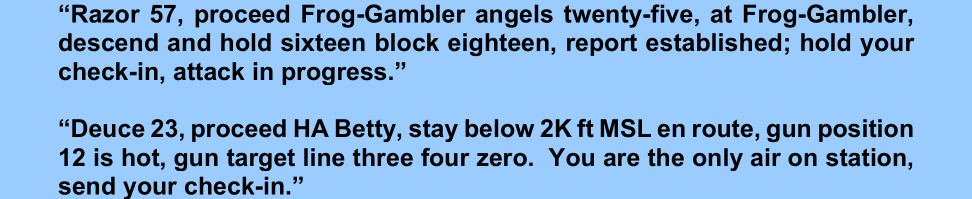
\includegraphics[width=\textwidth]{routing_ex5.png}
            \caption{Routing: information alliés.}
            \label{fig:routingallies}
        \end{figure}
    \ed
\ed

\section{Check-in}

\e
	\begin{minipage}{\linewidth}
    \item
    Le check-in est la première phase du \acrshort{cas} en tant que tel. C’est l’appel effectué de l’appareil en \acrshort{cas} vers le \acrshort{jtac}/\acrshort{faca} pour lui signifier qu’il est prêt à remplir sa mission de \acrshort{cas}.
    \item Comme le check-in peut prendre un certain temps, un appel préliminaire devrait être effectué. Par exemple:
	\begin{lstlisting}[caption=Appel préliminaire, label=preliminary_call]
    PIRATE, ici REDWOLF, pour check-in, quand dispo.
	\end{lstlisting}
	\end{minipage}

	\begin{minipage}{\linewidth}
    \item Format du check-in:
    \begin{figure}[H]
        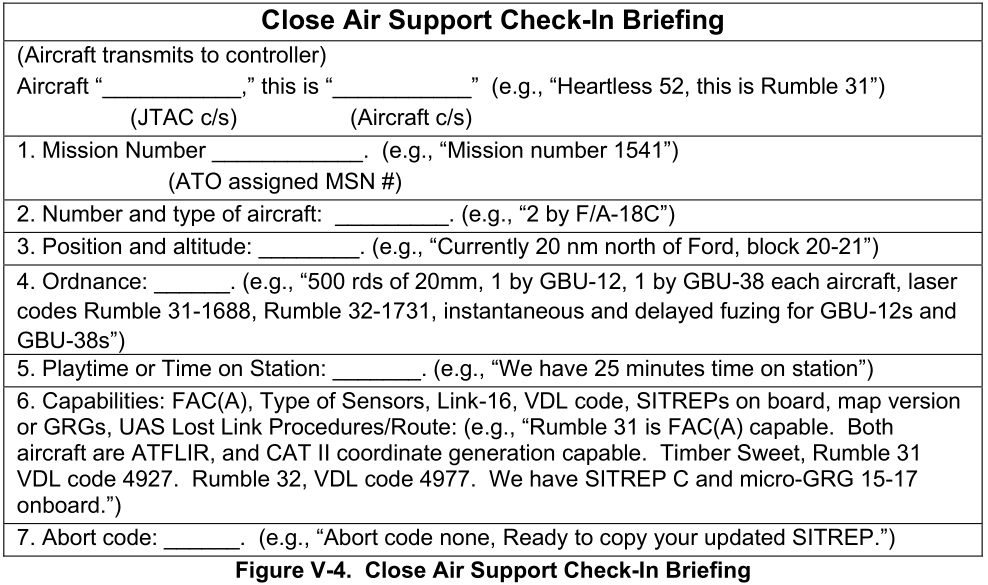
\includegraphics[width=\textwidth]{checkin.png}
        \caption{Format check-in.}
        \label{fig:checkin}
    \end{figure}    
    \end{minipage}
    
    \begin{minipage}{\linewidth}
    \item S'il le souhaite, le \gls{jtac}/\gls{faca} peut demander un check-in abrégé:
    \begin{figure}[H]
        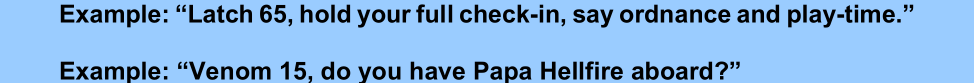
\includegraphics[width=\textwidth]{abbregcheckin.png}
        \caption{Format check-in abrégé.}
        \label{fig:abbregcheckin}
    \end{figure}
    \end{minipage}
    
    \item Le code d’annulation (ligne 7) est un code alphabétique servant à authentifier la directive “Abort” du J-TAC/FAC(A).
    
    \begin{minipage}{\linewidth}
    \item Exemple de check-in:
    \begin{lstlisting}[caption=Check-in, label=checkin]
	PIRATE ici REDWOLF
    	Mission 1234
	    2 Kamov
	    20km au sud de Poti, 500m MSL
    	24 Vikhrs, 80 roquettes, full guns
	    Playtime 30 minutes
    	Senseurs: Shkval
	    Abort code: X-RAY TANGO ZULU
	\end{lstlisting}
    \end{minipage}
\ed
